\section{Ensembles of Views for OOD Detection}
\label{sec:propwork-meo}

\begin{figure}
 \centering
 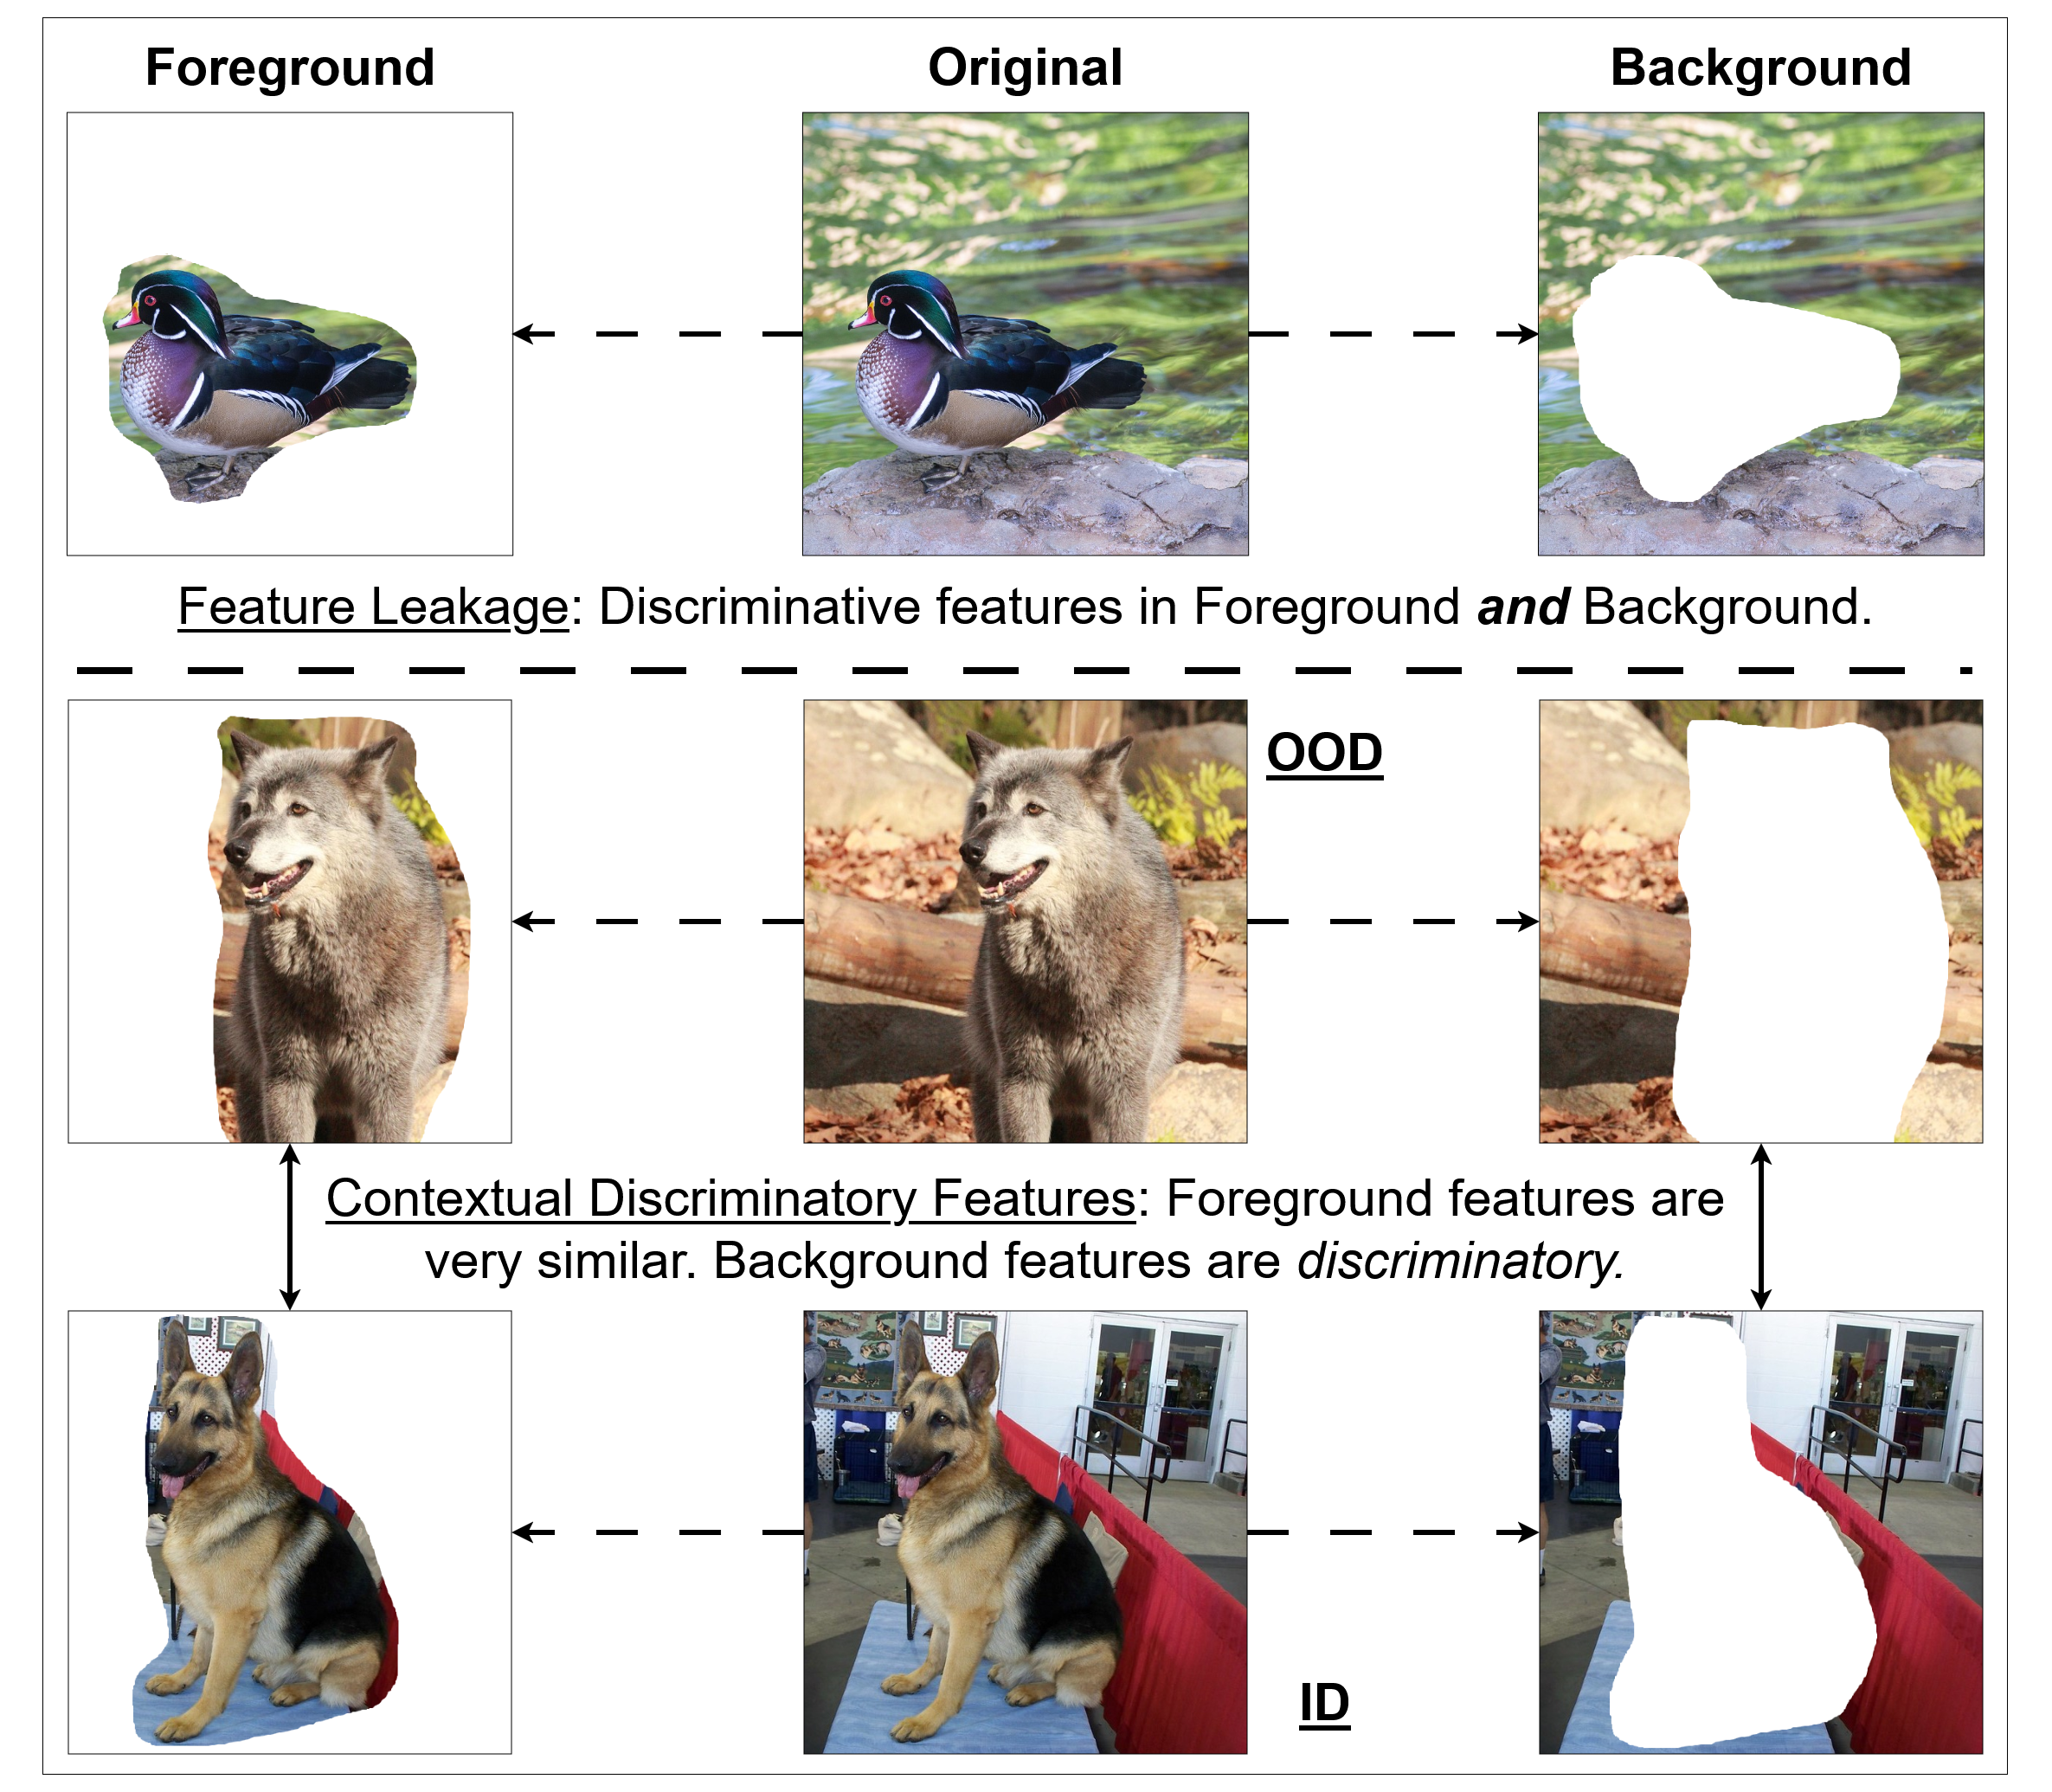
\includegraphics[width=1.\linewidth]{figures/meo_motivation}

  \caption{\sysa fails to account for samples that have ID class-relevant discriminative features in both the foreground \textit{and} the background (top row). Accounting for the discriminative features across foreground-background views in differing capacities is necessary for some near-OOD cases, such as that shown in the bottom section where the background features provide critical contextual information distinguishing the ``wolf'' from the ``dog''.
  }
  \label{fig:propwork-meo-motiv}
\end{figure}

%(shortcomings of MOD: unstable, selection can be easily biased towards/away from certain views) - covered in previous section

%(motivation: if we can train the mv model to extract helpful features from all views then we can include all of them)
%(motivation: also investigate which views are helpful at which points)

%The original motivation for \sysa was to identify and exclusively include whichever view (out of either the foreground or background views) contained more ID class-relevant discriminative features. However, there is no guarantee that such information is located exclusively in one of the views. 
MOD assumes that ID class-relevant discriminative features are exclusively in either the foreground or the background view. It selects one of these views using a view selector before combining it with the original image for OOD detection. However, this assumption is rarely valid. \ref{fig:propwork-meo-motiv} gives two examples where MOD fails to capture the entirety of discriminative features in either of the segmented view. In the first row, distinguishing components of the ``duck'' class are primarily in the foreground view but several important components are also in the background (e.g. the water and the reflections). In the lower section (second and third rows), the ID object discriminative features are all in the foreground views but important contextual features are in the background views. Domestic features in the background help contextualize the ID object of ``dog'' in the foreground against OOD object ``wolf'' which appears similar in the foreground but contains significantly different natural features in the background. Considering \emph{all views} in multi-view OOD detection can be beneficial.

%To investigate the benefits of considering \textit{all} views for OOD detection, the proposed method, \textbf{M}ulti-view \textbf{E}nsemble for \textbf{O}oD detection (\textbf{\sysb}), generates features for all individual views and all combinations of views before evaluating them in ensembles based on ID accuracy and OOD detection performance . Specifically, \sysb extracts view-specific features (called ``single-view features''), fused features of each pair of single-view features (``cross-view features''), and a fused feature of all single-view features (``comprehensive fused feature''). All of these individual and combination fused features are used to generate predictions, and the complete \sysb model is trained end-to-end using an aggregated loss (accounting for all feature predictions). The importance of each view in contributing discriminative features is evaluated through generation of all possible ensembles of learned individual and combination fused features during testing.
The proposed method, %\textbf{M}ulti-view \textbf{E}nsemble for \textbf{O}OD detection (\textbf{\sysb})
Multi-view Ensemble for OOD detection (MEO), investigates this approach by generating features for all possible combinations of views. This set of view combinations (including the views themselves) is systematically evaluated for ID accuracy and OOD detection performance. Specifically, MEO extracts view-specific features (``single-view features''), features fused from pairs of single-view features (``cross-view features''), and a cumulative feature resulting from the fusion of all single-view features (``comprehensive fused feature''). Each of these individual and fused features are learned end-to-end through an aggregate loss and used at test time for ID class prediction and feature-based OOD detection. All possible ensembles of individual and fused features are evaluated for contribution towards learning discriminative features and improving OOD detection.

\subsection{Proposed Method}
\label{sec:propwork-meo-propmeth}

%(proposed architecture with explanation)

%For \sysa, the FgBg multi-view model $f_{MV}$ is implemented using a multi-view convolutional NN (CNN), or MVCNN \cite{su2015multi}, as the backbone. The multi-view feature extractors are each a CNN feature extraction backbone parameterized by $\theta$, $\phi_v = f_{\theta,v}$. Each $f_{\theta,v}$ learn view feature vectors representative of ID class information, taking as input the corresponding view $x_v$ and outputting a $d$-dimensional feature vector $z_v \in \mathbb{R}^d$, $\phi_v: \mathcal{X} \mapsto \mathbb{R}^d$. Here, $V = \{org, fg, bg\}$, and the multi-view feature extractors $\phi_{MV}$ give $Z_{MV} = \{z_{org}, z_{fg}, z_{bg}\}$. The corresponding individual classification weight matrices $W_{MV}$ and biases $b_{MV}$ give $\hat{Y}_{MV} = \{\hat{y}_{org}, \hat{y}_{fg}, \hat{y}_{bg}\}$. In \sysa, the fusion component $\mathcal{U}$ is designed with a view selector, described below, and outputs $z_{\mathcal{U}}$ and $\hat{y}_{\mathcal{U}}$.
MEO resembles MOD in that an MVCNN is used for the FgBg multi-view model $f_{MV}$ backbone. Each feature extractor $\phi_v = f_{\theta,v}$ (parameterized by $\theta$) outputs a $d$-dimensional feature vector from input view $x_v$, $\phi_v: \mathcal{X} \mapsto \mathbb{R}^d$. The multi-view feature extractors $\phi_{MV}$ give $Z_{MV} = \{z_{org}, z_{fg}, z_{bg}\}$ with corresponding classification parameters $W_{MV}$ and $b_{MV}$ subsequently outputting $\hat{Y}_{MV} = \{\hat{y}_{org}, \hat{y}_{fg}, \hat{y}_{bg}\}$. The fusion component $\mathcal{U}$ in MEO differs significantly from MOD, instead constructing the single-view features, cross-view features, and comprehensive fused feature for ensembling.

\begin{figure}
 \centering
 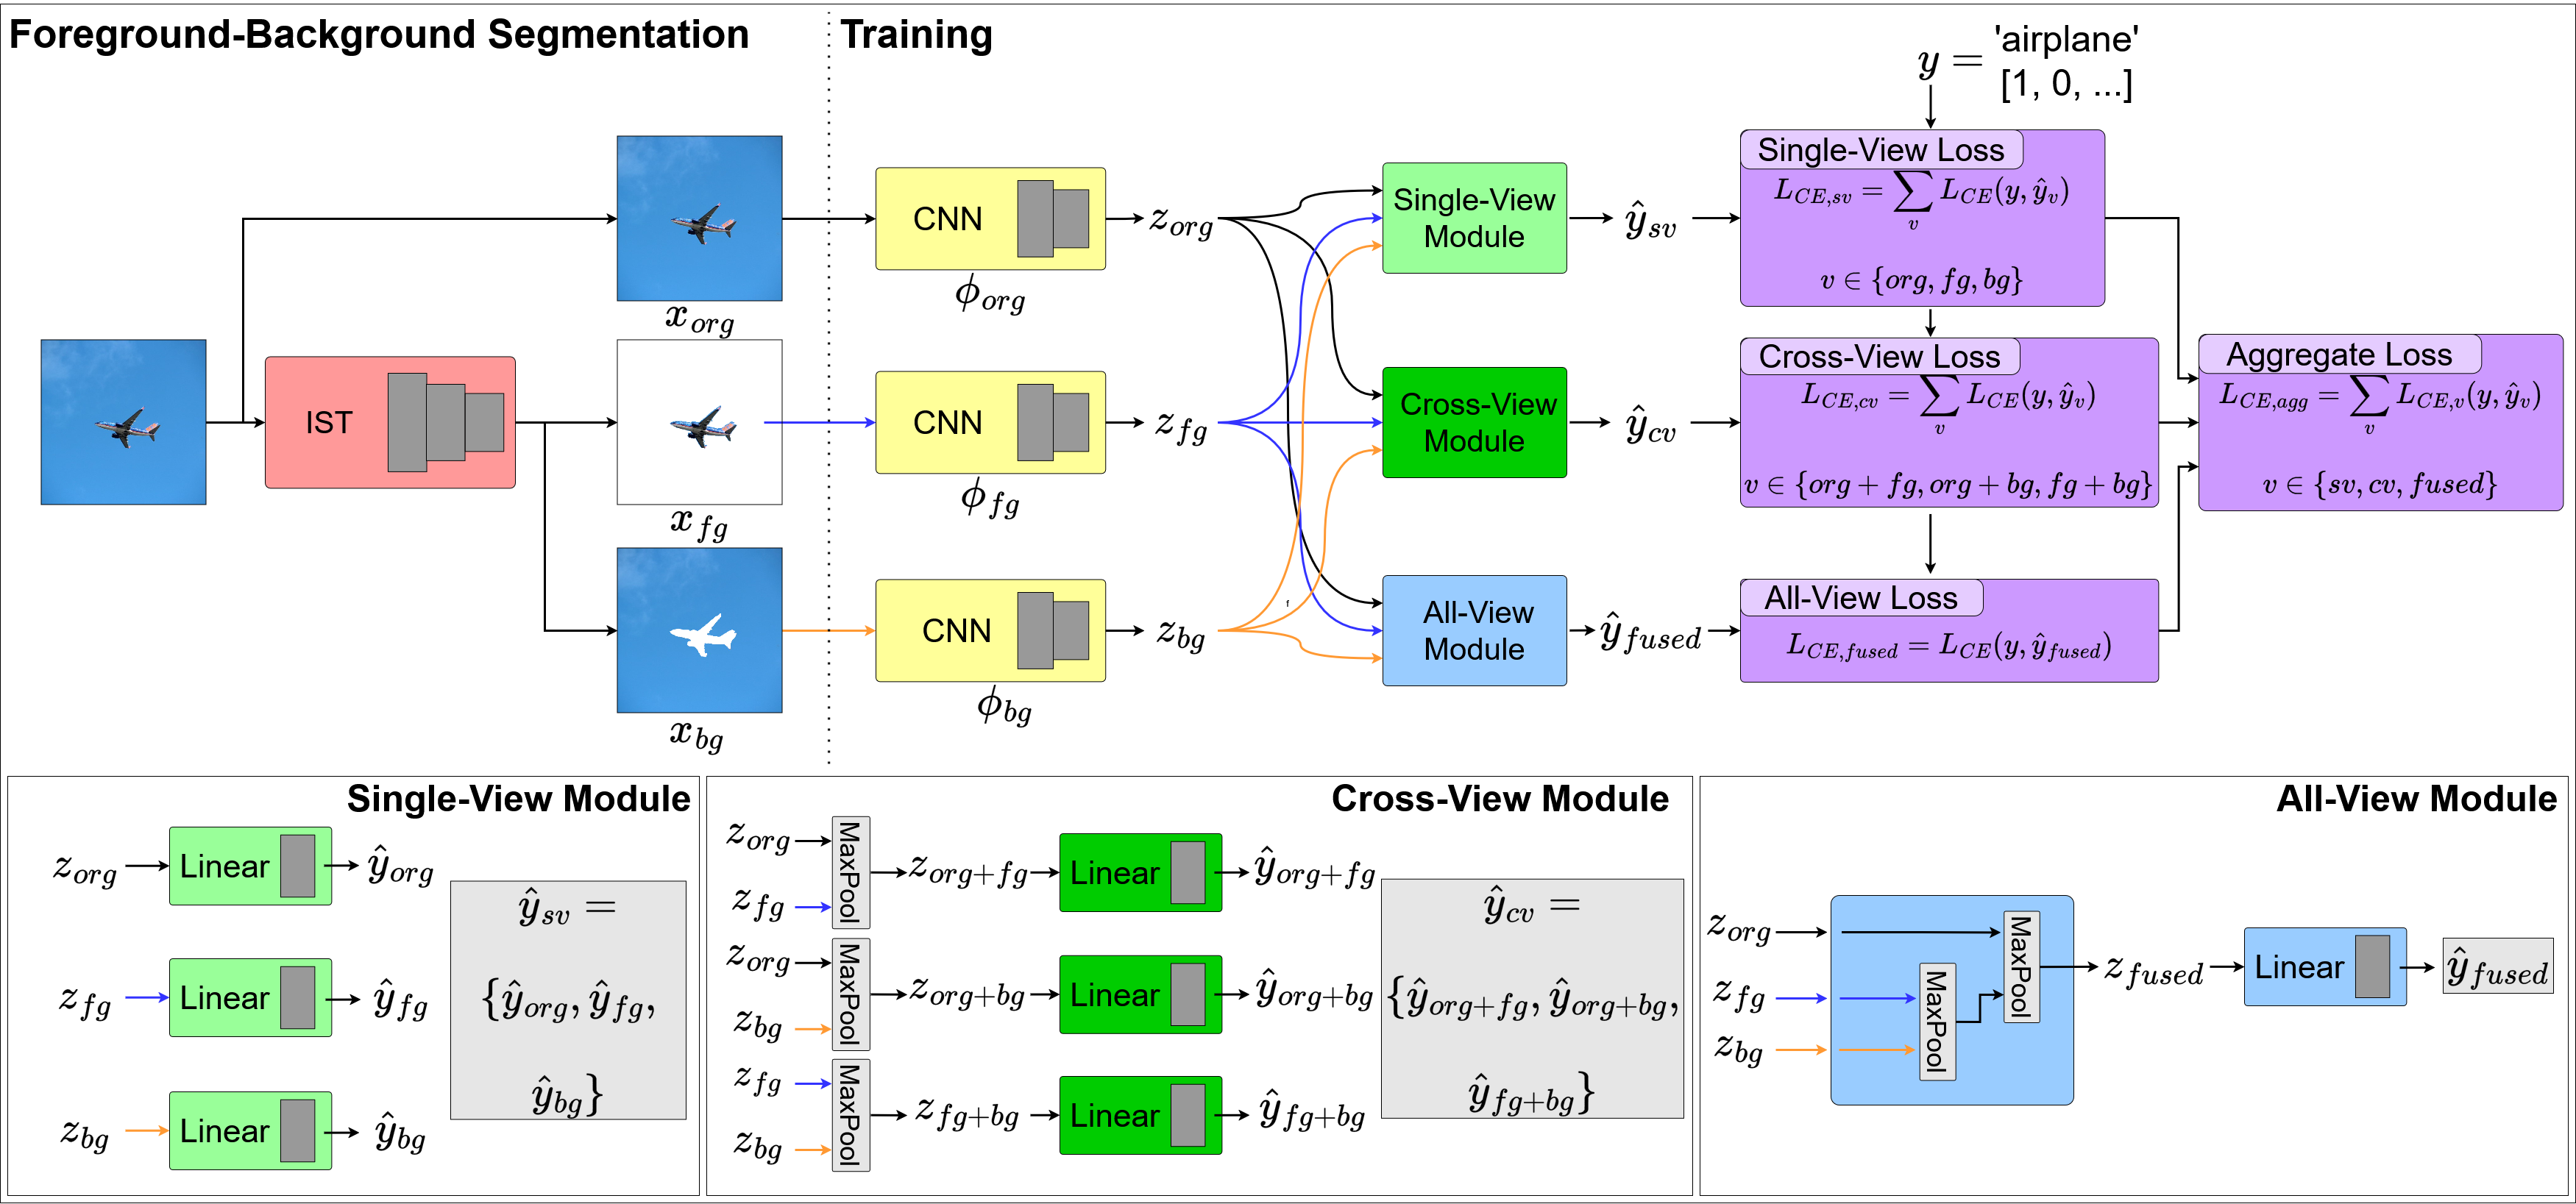
\includegraphics[width=1.\linewidth]{figures/meo_diagram}

  \caption{System diagram of the proposed \sysb. Forward pass is denoted by solid lines and backward pass follows the same lines in the reverse order until the dotted vertical line. %The original or fused image features are denoted by black lines. Foreground image features are denoted by blue lines, background image features are denoted by orange lines. 
  Best viewed in color.
  }
  \label{fig:propwork-meo-diagram}
\end{figure}

%Figure \ref{fig:propwork-meo-diagram} presents the architectural details of \sysb. Similar to \sysa, \sysb uses an MVCNN architecture with three view inputs and corresponding view feature extractors $\phi_{v}$ ($v \in \{org, fg, bg\}$). However, in \sysb the fusion module $\mathcal{G}$ is composed of three separate modules: the Single-View Module, the Cross-View \emph{feature fusion} Module, and the All-View \emph{feature fusion} Module. The Single-View Module does not perform feature fusion. Instead, each view-specific feature vector $z_{org}$, $z_{fg}$, $z_{bg}$ (the single-view features) is passed to a respective linear layer, resulting in three view-specific prediction logits $\hat{y}_{org}$, $\hat{y}_{fg}$, $\hat{y}_{bg}$ (the single-view logits). 
The flow of information for MEO is illustrated in  \ref{fig:propwork-meo-diagram}. The IST segments the original image view (\textit{org}) into a foreground view (\textit{fg}) and a background view (\textit{bg}). The MVCNN backbone generates features $Z_{MV}$ and logits $\hat{Y}_{MV}$. In MEO, the fusion component $\mathcal{U}_{\text{\sysb}}$ is composed of three modules.

\subsubsection{Fusion Component}
The first module in MEO $\mathcal{U}_{\text{\sysb}}$ is the Single-View Module which does not perform fusion, instead simply returning $Z_{MV}$ and $\hat{Y}_{MV}$ (i.e. a no-op).

%In the Cross-View Module, each possible pair of single-view feature vectors, i.e. $\{org+fg, org+bg, fg+bg\}$, is fused using max-pooling. For any two \emph{different} single-view features $z_{v1}$ and $z_{v2}$, the features are combined into a fused feature $z_{v12}$
%\begin{equation}
%\begin{aligned}
%    z_{v12} = \text{MaxPooling}_{p} \{z_{v1}, z_{v2}\}
%\end{aligned}
%\end{equation}
%Fusion in the Cross-View Module results in three cross-view feature vectors $z_{org+fg}$, $z_{org+bg}$, $z_{fg+bg}$. Each of these features is individually passed to respective linear layers, resulting in three cross-view prediction logits $\hat{y}_{org+fg}$, $\hat{y}_{org+bg}$, $\hat{y}_{fg+bg}$.
The second module is the Cross-View Module, in which each possible pair of view-specific feature vectors, $\{org+fg, org+bg, fg+bg\}$, is combined via a max-pooling operation. Given any two \emph{different} view-specific feature vectors $z_{v1}$ and $z_{v2}$, the cross-view feature vector $z_{v12}$ is
\begin{equation}
\begin{aligned}
    z_{v12} = \text{MaxPooling}_{d} \{z_{v1}, z_{v2}\}.
\end{aligned}
\end{equation}
The Cross-View Module in $\mathcal{U}_{\text{\sysb}}$ outputs three cross-view feature vectors $z_{org+fg}$, $z_{org+bg}$, $z_{fg+bg}$, each of which is passed to a respective linear layer with $W_{org+fg}$, $W_{org+bg}$, $W_{fg+bg}$ and $b_{org+fg}$, $b_{org+bg}$, $b_{fg+bg}$. This also results in cross-view predicted logits $\hat{y}_{org+fg}$, $\hat{y}_{org+bg}$, $\hat{y}_{fg+bg}$.

%Finally, the All-View Module uses consecutive max-pooling operations to combine all single-view feature vectors into a single comprehensive fused feature vector
%\begin{equation}
%\begin{aligned}
%    z_{fused} = \text{MaxPooling}_{p}\{z_{org},~\text{MaxPooling}_{p}\{z_{fg},~z_{bg}\}\}
%\end{aligned}
%\end{equation}
%The fused feature $z_{fused}$ is passed to a linear layer, resulting in the comprehensive fused prediction logits $\hat{y}_{fused}$.
The third and final module is the All-View Module. Consecutive max-pooling operations are used to combine all view-specific feature vectors into a single, fused feature vector containing comprehensive information across all views
\begin{equation}
\begin{aligned}
    z_{fused} = \text{MaxPooling}_{d}\{z_{org},~\text{MaxPooling}_{d}\{z_{fg},~z_{bg}\}\}.
\end{aligned}
\end{equation}
$z_{fused}$ is similarly passed to a respective linear layer $W_{fused}$, $b_{fused}$, resulting in $\hat{y}_{fused}$.

%The fusion module $\mathcal{G}$ for \sysb is the composition of all three Single-View, Cross-View, and All-View Modules. Thus the final outputs of the \sysb fusion module $\mathcal{G}$ are the single-view, cross-view, and comprehensive fused feature vectors $Z_{mv} = \{z_{org}, $ $z_{fg}, $ $z_{bg}, $ $z_{org+fg}, $ $z_{org+bg}, $ $z_{fg+bg}, $ $z_{fused}\}$ and the single-view, cross-view, and comprehensive fused prediction logits $\hat{Y}_{mv} = \{\hat{y}_{org}, $ $\hat{y}_{fg}, $ $\hat{y}_{bg}, $ $\hat{y}_{org+fg}, $ $\hat{y}_{org+bg}, $ $\hat{y}_{fg+bg}, $ $\hat{y}_{fused}\}$. For notation convenience, the feature sets are further delineated according to single-view features $z_{sv} = \{z_{org}, z_{fg}, z_{bg}\}$ and cross-view features $z_{cv} = \{z_{org+fg}, z_{org+bg}, z_{fg+bg}\}$.
%At no point in \sysb are the feature extractors frozen while the linear layers are learned (including in the above modules). The entirety of \sysb, i.e. both features and logits, is learned end-to-end.
In summary, the MEO fusion component $\mathcal{U}_{\text{\sysb}}$ utilizes the Single-View, Cross-View, and All-View Modules to output a set of feature vectors $Z_{\mathcal{U}} = \{z_{org}, $ $z_{fg}, $ $z_{bg}, $ $z_{org+fg}, $ $z_{org+bg}, $ $z_{fg+bg}, $ $z_{fused}\}$ and prediction logits $\hat{Y}_{\mathcal{U}} = \{\hat{y}_{org}, $ $\hat{y}_{fg}, $ $\hat{y}_{bg}, $ $\hat{y}_{org+fg}, $ $\hat{y}_{org+bg}, $ $\hat{y}_{fg+bg}, $ $\hat{y}_{fused}\}$. For convenience, feature sets are further delineated according to view-specific features $z_{sv} = \{z_{org}, z_{fg}, z_{bg}\}$ and cross-view features $z_{cv} = \{z_{org+fg}, z_{org+bg}, z_{fg+bg}\}$.

%\textbf{Training:} \sysb is trained end-to-end using a view-aggregate loss $\mathcal{L}_{CE,agg}$ which aggregates the CE losses of all single-view, cross-view, and comprehensive fused predictions.
%
%Given a one-hot true label vector $y$, $\mathcal{L}_{CE,agg}$ is formulated as follows. First, the view-specific CE loss $\mathcal{L}_{CE,sv}$ is defined for each single view $sv \in \{org, fg, bg\}$
%\begin{equation}
%\begin{aligned}
%    \mathcal{L}_{CE,sv}(y, \hat{y}_{sv}) & = -\sum_{c \in \mathcal{Y}} y_{c} \log(\hat{y}_{sv,c}) \\
%\end{aligned}
%\end{equation}
%where $\hat{y}_{sv,c}$ is the logit value of $\hat{y}_{sv}$ for class $c$.
%
%The CE losses for each cross-view $\mathcal{L}_{CE,cv}$, $cv \in \{org+fg, org+bg, fg+bg\}$, is defined similarly
%\begin{equation}
%\begin{aligned}
%    \mathcal{L}_{CE,cv}(y, \hat{y}_{cv}) & = -\sum_{c \in \mathcal{Y}} y_{c} \log(\hat{y}_{cv,c}) \\
%\end{aligned}
%\end{equation}
%
%The comprehensive fused CE loss $\mathcal{L}_{CE,fused}$ is the CE loss of the comprehensive fused prediction logits
%\begin{equation}
%\begin{aligned}
%    \mathcal{L}_{CE,fused}(y, \hat{y}_{fused}) & = -\sum_{c \in \mathcal{Y}} y_{c} \log(\hat{y}_{fused,c}) \\
%\end{aligned}
%\end{equation}
%
%The final aggregate CE loss $\mathcal{L}_{CE,agg}$ is the sum of the above losses
%\begin{equation}
%\begin{aligned}
%    %~org+fg, ~org+bg, ~fg+bg\}}}} \mathcal{L}_{CE,v} (y, \hat{y}_{v})
%    \mathcal{L}_{CE,agg} & = \mathcal{L}_{CE,sv} (y, \hat{y}_{sv}) + \mathcal{L}_{CE,cv} (y, \hat{y}_{cv}) + \mathcal{L}_{CE,fused} (y, \hat{y}_{fused})
%\end{aligned}
%\end{equation}
\subsubsection{Training}
The MEO model is learned end-to-end using a view-aggregate loss $\mathcal{L}_{CE,agg}$. The loss aggregates the classification losses of all single-view, cross-view, and comprehensive fused feature-based predictions. At no point is any component or set of parameters in MEO frozen while other parameters are trained.

A one-hot true label vector $y$ is used to train MEO via $\mathcal{L}_{CE,agg}$ through each set of view features. Specifically, a view-specific CE loss $\mathcal{L}_{CE,sv}$ is defined for each $sv \in \{org, fg, bg\}$
\begin{equation}
\begin{aligned}
    \mathcal{L}_{CE,sv}(y, \hat{y}_{sv}) & = -\sum_{c \in \mathcal{Y}} y_{c} \log(\hat{y}_{sv,c}). \\
\end{aligned}
\end{equation}
$\hat{y}_{sv,c}$ is the logit value of $\hat{y}_{sv}$ for class $c$.

Cross-views $cv \in \{org+fg, org+bg, fg+bg\}$ are accounted for through CE loss $\mathcal{L}_{CE,cv}$
\begin{equation}
\begin{aligned}
    \mathcal{L}_{CE,cv}(y, \hat{y}_{cv}) & = -\sum_{c \in \mathcal{Y}} y_{c} \log(\hat{y}_{cv,c}). \\
\end{aligned}
\end{equation}

The comprehensive fused information is accounted for through CE loss $\mathcal{L}_{CE,fused}$
\begin{equation}
\begin{aligned}
    \mathcal{L}_{CE,fused}(y, \hat{y}_{fused}) & = -\sum_{c \in \mathcal{Y}} y_{c} \log(\hat{y}_{fused,c}). \\
\end{aligned}
\end{equation}

These CE losses are combined in the final aggregate CE loss $\mathcal{L}_{CE,agg}$
\begin{equation}
\begin{aligned}
    %~org+fg, ~org+bg, ~fg+bg\}}}} \mathcal{L}_{CE,v} (y, \hat{y}_{v})
    \mathcal{L}_{CE,agg} & = \mathcal{L}_{CE,sv} (y, \hat{y}_{sv}) + \mathcal{L}_{CE,cv} (y, \hat{y}_{cv}) + \mathcal{L}_{CE,fused} (y, \hat{y}_{fused}).
\end{aligned}
\end{equation}

%\textbf{OOD Detection:} \sysb uses the MD OOD score for the same reasons as \sysa, i.e. the use of multiple views constructs a rich feature space specially suited for distance-based OOD detection methods. Note that while only MD is considered in this proposed work as a representative technique, \sysb is compatible with other distance-based OOD detection methods as well.
%
%The definition of MD for \sysb is identical to that of \sysa (see Section \ref{sec:propwork-mod-propmeth}). However, instead of only generating empirical class means and a covariance matrix for the comprehensive fused feature $z_{fused}$, \sysb calculates empirical class means $\hat{\mu}_{c,v}$ and covariance matrices $\hat{\Sigma}_{v}$ for each view feature $v \in \{org, fg, bg, org+fg, org+bg, fg+bg, fused\}$. Given a test instance $x'$, \sysb extracts the feature vector $z'_{v}$ and computes the distance between it and the nearest class-conditional Gaussian distribution for the view $v$. The negative of this distance is the final OOD score for view $v$
%\begin{equation}
%\begin{aligned}
%    M_{MD,v}(x') = \max_{c} (-(z_{v}' - \hat{\mu}_{c,v})^\top \hat{\Sigma}_{v}^{-1} (z_{v}' - \hat{\mu}_{c,v})) \\
%\end{aligned}
%\end{equation}
\subsubsection{OOD Detection}
Following from MOD (see Section \ref{sec:propwork-mod-propmeth}), MEO leverages distance-based OOD detection methods to exploit the rich feature space learned from the use of foreground-background segmented views. MEO is compatible with all distance-based (and otherwise post-hoc) OOD detection methods that operate on features and/or logits. However, this work only presents results for MD.

The implementation of MD for MEO is very similar to that in MOD. However, given that MEO uses a combination of view-specific features, cross-view features, and a comprehensive fused feature, multiple empirical class means and covariance matrices must be defined. MEO calculates empirical class means $\hat{\mu}_{C,v}$ and covariance matrices $\hat{\Sigma}_{v}$ for each view feature $v \in \{org, fg, bg, org+fg, org+bg, fg+bg, fused\}$. A test sample $x'$ is processed by MEO into feature vector $z'_{v}$. Distances are computed between $z'_{v}$ and the nearest class-conditional Gaussian distribution for view $v$. The negative distance is the OOD score for view $v$
\begin{equation}
\begin{aligned}
    S_{MD,v}(x') = \max_{c} (-(z_{v}' - \hat{\mu}_{c,v})^\top \hat{\Sigma}_{v}^{-1} (z_{v}' - \hat{\mu}_{c,v})). \\
\end{aligned}
\end{equation}

%(ensembles definitions)

\subsubsection{Single-, Cross-, and Comprehensive Fused View Ensembling}

%During testing, all possible combinations of view feature vectors, i.e. $z_{sv}$, $z_{cv}$, and $z_{fused}$, and prediction logits, i.e. $\hat{y}_{sv}$, $\hat{y}_{cv}$, and $\hat{y}_{fused}$, are considered. An ensemble $E$ is defined as the combination of view members, i.e. $E \subseteq \{org, fg, bg, org+fg, org+bg, fg+bg, fused\}$. Any given ensemble $E$ has access to all prediction logits $\hat{y}_{e}$ and MD OOD scores $M_{MD,e}$ for its members $e \in E$.
All possible combinations of MEO feature vectors $z_{sv}$, $z_{cv}$, $z_{fused}$ and prediction logits $\hat{y}_{sv}$, $\hat{y}_{cv}$, and $\hat{y}_{fused}$ are considered during test-time evaluation. An ensemble $\mathcal{E}$ is defined as the set of members composed of views, $\mathcal{E} \subseteq \{org, fg, bg, org+fg, org+bg, fg+bg, fused\}$. An ensemble $\mathcal{E}$ outputs prediction logits $\hat{y}_{e}$ and MD OOD scores $S_{MD,e}$ for each member $e \in \mathcal{E}$.

%For ID classification, \sysb combines all ensemble $E$'s members prediction logits $\hat{y}_{e}$ by applying a softmax operation on each ensemble member $e$'s logits before taking the element-wise product of all resultant prediction distributions
%\begin{equation}
%\begin{aligned}
%    \hat{y}_{ens} & = \prod_{e ~\in~ E} \sigma(\hat{y}_{e}) \\
%\end{aligned}
%\end{equation}
%where $\hat{y}_{ens}$ is a vector representing the final ensemble prediction result and $\sigma(\hat{y}_{e})$ is the softmax operation on each ensemble member prediction logits $\hat{y}_{e}$.
\subsubsection{Ensemble ID Classification}
MEO combines all ensemble $\mathcal{E}$'s member prediction through element-wise product of all softmax logits $\text{softmax}(\hat{y}_{e})$
\begin{equation}
\begin{aligned}
    \hat{y}_{\mathcal{E}} & = \prod_{e ~\in~ \mathcal{E}} \text{softmax}(\hat{y}_{e}). \\
\end{aligned}
\end{equation}
Note that $\hat{y}_{\mathcal{E}}$ is the final prediction vector for ensemble $\mathcal{E}$ resulting from the combination of all member prediction distributions. %$\text(softmax)$ is the softmax operation on a vector.

%For OOD detection, \sysb takes the mean across all ensemble $E$'s members MD OOD scores $M_{MD,e}(x')$ for a given test instance $x'$
%\begin{equation}
%\begin{aligned}
%    M_{MD,ens}(x') & = \frac{1}{\lvert E \rvert} \sum_{e ~\in~ E} M_{MD,e}(x') \\
%\end{aligned}
%\end{equation}
%where $M_{MD,ens}$ is the final ensemble MD OOD score.
%
%It is important to note that the cross-view features and predictions are \emph{not} simply degenerate ensembles of their components, e.g. $z_{fg+bg}$ is not semantically identical to the ensemble of $z_{fg}$ and $z_{bg}$. Each view feature is trained using a separate linear layer prediction head and is a unique fusion of its single-view feature components. Therefore, the cross-view feature vectors encode unique data relevant to both the view itself and the data sample.
\subsubsection{Ensemble OOD Detection}
The ensemble $\mathcal{E}$ OOD score is the mean across all member MD OOD scores $S_{MD,e}(x')$ for test sample $x'$
\begin{equation}
\begin{aligned}
    S_{MD,\mathcal{E}}(x') & = \frac{1}{\lvert \mathcal{E} \rvert} \sum_{e ~\in~ \mathcal{E}} S_{MD,e}(x'). \\
\end{aligned}
\end{equation}
Note that $S_{MD,\mathcal{E}}$ is the final OOD score for ensemble $\mathcal{E}$.

Cross-view features and predictions semantically represent more than their separate components. For example, $z_{fg+bg}$ is not identical to the ensemble $\mathcal{E} = \{z_{fg}, z_{bg}\}$. Each view (single-view, cross-view, or comprehensive fused) is trained using a distinct prediction linear layer on top of being a unique fusion of view-specific components. Thus, cross-view feature vectors contain unique discriminative feature information relevant to the ID class.

\subsection{Experiments}
\label{sec:propwork-meo-exp}

%(CIFAR-100 results: near- and far-ood)

%The evaluation of \sysb follows a nearly identical experimental setup as that of \sysa. Deviations are described accordingly in each relevant section.
The experimental settings from MOD are used for MEO, with minor deviations (noted where appropriate). %Full results on all possible ensembles $\mathcal{E}$ are presented in the Appendix (see Appendix Section \ref{}{\color{red}TODO}).

%\textbf{Datasets:} CIFAR-100 \cite{krizhevsky2009learning} remains as the training and ID testing dataset. The SVHN \cite{yuval2011reading} dataset is added as a far-OOD dataset.
\subsubsection{Datasets}
CIFAR-10 and CIFAR-100 \cite{krizhevsky2009learning} are used as training and ID testing datasets. SVHN \cite{yuval2011reading} is added as a far-OOD dataset. ImageNet-30 \cite{russakovsky2015imagenet} is also added as a training and ID testing dataset. OOD datasets for ImageNet-30 follow previous experimental work \cite{li2023rethinking,yang2022openood} and include CIFAR-10, CIFAR-100, SVHN, LSUN, Textures, Places365, iNaturalist, and Tiny ImageNet. ImageNet-30 is not used as an OOD dataset for the CIFAR ID experimental settings because it has significantly higher resolution and image size, making the data domains incomparable.

%\textbf{Baselines:} Additional state-of-the-art baselines were included for the \sysb experiments: Optimal Parameter and Neuron Pruning (OPNP) \cite{chen2024optimal}, Orthogonal Gradient Projection (GradOrth) \cite{behpour2024gradorth}, and Adaptive Temperatue Scaling (ATS) \cite{krumpl2024ats}. Their results are directly copied from the respective papers as none of them provide code for reproduction and their experimental setups are the same.
\subsubsection{Baselines}
For MEO experiments, additional state-of-the-art baseline methods were considered. Specifically, Optimal Parameter and Neuron Pruning (OPNP) \cite{chen2024optimal}, Orthogonal Gradient Projection (GradOrth) \cite{behpour2024gradorth}, and Adaptive Temperatue Scaling (ATS) \cite{krumpl2024ats} were included based on their recent results. Results for these additional baselines are copied from respective papers, as their experimental setups are the same and code was either not available or failed to converge.

\subsection{Results}
\label{sec:propwork-meo-results}

%((if space) VERY BASIC analysis/conclusions on results)

\begin{table*}
\small
\centering
\caption{CIFAR-10 ID classification (\textbf{Accuracy}) and OOD detection performance (\textbf{AUC}) comparison between top-3 \sysb ensembles and recent state-of-the-art baselines on \textit{near-OOD} datasets. %All numeric values are percentages. Best results are emphasized with \textbf{boldface}. 
The following key is used to shorten ensemble members: ``\textbf{f}'' - comprehensive fused feature/logits, ``\textbf{O}'' - original single-view, ``\textbf{F}'' - foreground single-view, ``\textbf{B}'' - background single-view, ``\textbf{OF}'' - $org+fg$ cross-view, ``\textbf{OB}'' - $org+bg$ cross-view, and ``\textbf{FB}'' - $fg+bg$ cross-view. For example, a ``f+OF+OB'' ensemble would have members $\{fused$, $org+fg$, $org+bg\}$. This notation is used consistently throughout the rest of the dissertation with respect to \sysb.
}
\vspace{0.1cm}
\scalebox{1.0}{
\begin{tabular}{|l|c|ccc|}
\hline
\multicolumn{1}{|c|}{\multirow{2}{*}{}} & ID & \multicolumn{3}{c|}{OOD}    \\ \cline{2-5} 
\multicolumn{1}{|l|}{} & CIFAR-10   & CIFAR-100  & Tiny ImageNet  & \multicolumn{1}{|c|}{Average}   \\ \hline
MSP       & 94.73$_{\pm 0.11}$ &  87.05$_{\pm 0.51}$   &  \multicolumn{1}{c|}{87.98$_{\pm 0.34}$}   & 87.51  \\  
KNN       & 94.73$_{\pm 0.11}$ & 89.55$_{\pm 0.22}$   &  \multicolumn{1}{c|}{90.15$_{\pm 0.14}$}   &  89.85  \\  
MD        & 94.73$_{\pm 0.11}$ & 83.33$_{\pm 0.72}$   &  \multicolumn{1}{c|}{83.68$_{\pm 0.68}$}   &   83.51 \\  
ViM       & 94.73$_{\pm 0.11}$ &  86.39$_{\pm 1.72}$   &  \multicolumn{1}{c|}{87.26$_{\pm 1.56}$}   &  86.82 \\ 
React     & 94.73$_{\pm 0.11}$ &  84.82$_{\pm 1.39}$   &  \multicolumn{1}{c|}{86.76$_{\pm 0.98}$}   &   85.79  \\  
FeatNorm  & 94.73$_{\pm 0.11}$ & 88.89$_{\pm 0.66}$  & \multicolumn{1}{c|}{90.16$_{\pm 0.81}$}   &  89.53   \\  
GEN       & 94.73$_{\pm 0.11}$ & 87.19$_{\pm 0.58}$   &  \multicolumn{1}{c|}{88.56$_{\pm 0.40}$}   &   87.87 \\  
LogitNorm & 94.56$_{\pm 0.22}$ & 90.80$_{\pm 0.82}$ &  \multicolumn{1}{c|}{91.80$_{\pm 0.65}$}   &   91.30 \\
CSI       & / &  92.2  &  97.6  & \multicolumn{1}{|c|}{94.90}  \\  
CMG-e     & / & 89.3 &  95.2  & \multicolumn{1}{|c|}{92.25} \\ \hline
MOD-MD  & 95.37$_{\pm 0.29}$ & 95.54$_{\pm 5.39}$ & \multicolumn{1}{c|}{96.34$_{\pm 2.60}$}  & 95.94  \\ \cdashline{1-5}
MEO-MD & & & & \multicolumn{1}{|c|}{} \\ %\cline{1-1} %\hline
f+O+F+OB    & 95.08$_{\pm 0.40}$ & \textbf{99.28$_{\pm 0.64}$} & 98.60$_{\pm 1.56}$ &  \multicolumn{1}{|c|}{\textbf{98.94}} \\ 
f+O+F+OF+OB & 94.95$_{\pm 0.34}$ & 99.00$_{\pm 0.52}$ & \textbf{98.76$_{\pm 1.45}$} &  \multicolumn{1}{|c|}{98.88}  \\ 
f+F+B+OB+FB & \textbf{95.24$_{\pm 0.39}$} & 99.09$_{\pm 0.64}$ & 98.50$_{\pm 1.59}$ &  \multicolumn{1}{|c|}{98.80}  \\ \hline
\end{tabular}
}
\label{tab:propwork-meo-results-cifar10-near}
\end{table*}

\begin{table*}
\small
\centering
\caption{CIFAR-10 OOD detection performance (\textbf{AUC}) comparison between top-3 \sysb ensembles and recent state-of-the-art baselines on \textit{far-OOD} datasets. %All numeric values are percentages. Best results are emphasized with \textbf{boldface}.
}
\vspace{0.1cm}
\scalebox{0.875}{
\begin{tabular}{|l|cccccc|}
\hline
\multicolumn{1}{|l|}{\multirow{2}{*}{}} &   \multicolumn{6}{c|}{OOD}   \\ \cline{2-7}
\multicolumn{1}{|l|}{}   &  SVHN &   LSUN & Textures  & Places365 & iNaturalist & \multicolumn{1}{|c|}{Average}  \\ \hline
MSP    & 93.39$_{\pm 2.30}$ &  90.45$_{\pm 0.42}$  & 92.01$_{\pm 0.58}$  & 89.88$_{\pm 0.55}$  & \multicolumn{1}{c|}{90.20$_{\pm 0.73}$}   & 91.18  \\  
KNN    & 95.45$_{\pm 1.38}$   &  92.29$_{\pm 0.15}$   & 94.24$_{\pm 0.40}$   & 91.46$_{\pm 0.25}$   & \multicolumn{1}{c|}{91.73$_{\pm 0.62}$}  & 93.03  \\  
MD     & 99.10$_{\pm 0.46}$  & 85.48$_{\pm 0.74}$ & 96.81$_{\pm 0.32}$   & 82.77$_{\pm 0.80}$ & \multicolumn{1}{c|}{87.31$_{\pm 1.57}$}  &  90.30   \\  
ViM    & 97.57$_{\pm 2.24}$   & 89.26$_{\pm 2.05}$ & 96.05$_{\pm 1.04}$ & 88.05$_{\pm 1.96}$ & \multicolumn{1}{c|}{89.96$_{\pm 1.27}$}   & 92.18   \\  
React  & 93.80$_{\pm 1.75}$ &  91.47$_{\pm 0.55}$   & 90.67$_{\pm 0.89}$   & 89.57$_{\pm 1.11}$   & \multicolumn{1}{c|}{87.94$_{\pm 2.30}$}   &  90.69  \\  
FeatNorm   & 99.07$_{\pm 0.40}$ & 91.93$_{\pm 1.15}$  & 94.61$_{\pm 0.23}$   & 95.37$_{\pm 0.41}$   & \multicolumn{1}{c|}{94.14$_{\pm 1.31}$}  &  95.03  \\  
GEN         & 94.15$_{\pm 2.17}$  &  91.35 $_{\pm 0.53}$  & 92.53$_{\pm 0.79}$   & 90.82$_{\pm 0.65}$  & \multicolumn{1}{c|}{90.97$_{\pm 0.90}$}   &  91.96   \\  
LogitNorm & 97.61$_{\pm 0.92}$  &  95.06$_{\pm 0.59}$  & 94.53$_{\pm 1.07}$  & 95.66$_{\pm 0.42}$   & \multicolumn{1}{c|}{93.18$_{\pm 1.05}$}   &   95.21  \\
OPNP       &  \textbf{99.90} &  /  & 98.20  & 97.64  & \multicolumn{1}{c|}{/}   &   /  \\ 
GradOrth  &  98.72 & / & 94.77  & 91.64   & \multicolumn{1}{c|}{/}   &   / \\ \hline
MOD-MD  & / & 96.02$_{\pm 2.97}$ & 98.42$_{\pm 1.12}$ & 95.90$_{\pm 3.04}$ & 98.63$_{\pm 0.57}$ & \multicolumn{1}{|c|}{97.24} \\ \cdashline{1-7}
MEO-MD & & & & & & \multicolumn{1}{|c|}{}  \\
f+O+F+OB    & 97.67$_{\pm 2.61}$ & 99.29$_{\pm 0.53}$ & 99.87$_{\pm 0.10}$ & 99.62$_{\pm 0.30}$ & \textbf{99.97$_{\pm 0.02}$} &  \multicolumn{1}{|c|}{99.29}    \\ 
f+O+F+OF+OB  & 98.34$_{\pm 1.22}$ & \textbf{99.40$_{\pm 0.43}$} & \textbf{99.90$_{\pm 0.09}$} & \textbf{99.66$_{\pm 0.22}$} & \textbf{99.97$_{\pm 0.02}$} &  \multicolumn{1}{|c|}{\textbf{99.45}}      \\ 
f+F+B+OB+FB & 97.74$_{\pm 2.17}$  &  99.19$_{\pm 0.56}$ & 99.86$_{\pm 0.10}$ & 99.49$_{\pm 0.33}$ & 99.96$_{\pm 0.03}$ &  \multicolumn{1}{|c|}{99.25}       \\  \hline
\end{tabular}
}
\label{tab:propwork-meo-results-cifar10-far}
\end{table*}

%\begin{figure}[tb]
%  \center
%\includegraphics[width=0.82\linewidth]{figures/mvens_view_distances}
%  \caption{
%  MDs for ID test (CIFAR-100) and OOD (Tiny ImageNet) data for each single-view. The distances for $B$ are 1) significantly larger than that of either $O$ or $F$ for OOD data, and 2) significantly larger for the OOD data than that of the ID data. Note that the data samples are sorted according to their MD distances from large to small. 
%  }
%  \vspace{-4mm}
%  \label{fig:propwork-meo-results-fgbg_contrib}
%\end{figure}

%Results of the \sysb experiments are shown in Table \ref{tab:propwork-meo-results-cifar100-far} (far-OOD datasets) and Table \ref{tab:propwork-meo-results-cifar100-near} (near-OOD datasets). To conserve space, only the top-3 \sysb ensembles are presented. %The full tables containing results for all possible \sysb ensembles is provided in \textcolor{blue}{TODO - ref to additional results... should we? or leave that for future work?}. 
%\sysb substantially outperforms state-of-the-art baselines in OOD detection. For far-OOD datasets (Table \ref{tab:propwork-meo-results-cifar100-far}), all \sysb ensembles improve the average AUROC (maximum improvement of 16.40\%) as well as the AUROC of each individual OOD dataset except SVHN. For near-OOD datasets (Table \ref{tab:propwork-meo-results-cifar100-near}), \sysb ensembles again outperform baselines, with the $f+O+F+OF+OB$ ensemble improving average AUROC by 9.82\%, CIFAR-10 AUROC by 2.93\%, and Tiny ImageNet AUROC by 9.51\%. \sysb also benefits ID classification, with all top-3 \sysb ensembles improving accuracy (maximum improvement of 0.97\%). An interesting observation from the top \sysb ensembles is that each ensemble includes at least one single-view feature, at least one cross-view feature, and the comprehensive fused feature. This suggests that all of the individual and combination fused features contain discriminative features important to representing ID class-relevant information and distinguishing OOD instances.
\ref{tab:propwork-meo-results-cifar10-near} (near-OOD datasets) and \ref{tab:propwork-meo-results-cifar10-far} (far-OOD datasets) show results for the MEO experiments on CIFAR-10. Only the top-3 MEO ensembles are presented in this section. Previous state-of-the-art baselines are unable to outperform MEO in OOD detection. 
In the near-OOD domain (\ref{tab:propwork-meo-results-cifar10-near}), the top MEO ensembles outperform all baselines. In particular, the $f+O+F+OB$ ensemble improves the average AUC by 4.04\%, AUC of CIFAR-100 by 7.08\%, and AUC of Tiny ImageNet by 1.00\%. Across the top-3 ensembles, performance is consistent. Variance of AUC is only 0.02\% for CIFAR-100, 0.02\% for Tiny ImageNet, and 0.005\% on average. MEO ensembles also outperform MOD, validating the idea of utilizing feature information in \emph{all} views for OOD detection instead of selectively eliminating views. The $f+O+F+OB$ MEO ensemble improves the average CIFAR-10 near-OOD AUC by 3.00\%, from 95.94\% to 98.94\%, a significant margin.
In the far-OOD domain (\ref{tab:propwork-meo-results-cifar10-far}), MEO ensembles again improve AUC both on average (4.24\%) and across individual datasets (except SVHN), where the $f+O+F+OF+OB$ ensemble underperforms by only 1.56\% (and still achieves a high AUC of 98.34\%). On the challenging iNaturalist far-OOD dataset, MEO ensembles perform extremely well, each improving AUC by 5.81-5.82\% over the nearest state-of-the-art baseline. Variance across the top-3 MEO ensembles is again low, only 0.01\% for average OOD detection performance. Similar to the near-OOD CIFAR-10 datasets, MEO ensembles improve on MOD, improving average OOD detection by 2.21\% and demonstrating a particularly large increase in Places365 of 3.76\%.
ID classification is also unaffected by the multi-view paradigm. All 3 top MEO ensembles improve ID classification accuracy (maximum improvement of 0.68\%), demonstrating that MEO is able to learn ID class-relevant discriminative features effective for OOD detection while maintaining ID classification functionality.

\begin{table*}
\small
\centering
\caption{CIFAR-100 ID classification (\textbf{Accuracy}) and OOD detection performance (\textbf{AUC}) comparison between top-3 \sysb ensembles and recent state-of-the-art baselines on \textit{near-OOD} datasets. %All numeric values are percentages. Best results are emphasized with \textbf{boldface}.
}
\vspace{0.1cm}
\scalebox{1.0}{
\begin{tabular}{|l|c|ccc|}
\hline
\multicolumn{1}{|c|}{\multirow{2}{*}{}} & ID &  \multicolumn{3}{c|}{OOD}    \\ \cline{2-5} 
\multicolumn{1}{|l|}{} & CIFAR-100  & CIFAR-10 & Tiny ImageNet & \multicolumn{1}{|c|}{Average}   \\ \hline
MSP       & 77.66$_{\pm 0.43}$  &  78.99$_{\pm 0.20}$  & \multicolumn{1}{c|}{80.74$_{\pm 0.26}$}  &  79.87 \\  
KNN       &  77.66$_{\pm 0.43}$ &  77.42$_{\pm 0.36}$ & \multicolumn{1}{c|}{81.67$_{\pm 0.16}$}   &   79.54 \\  
MD        &   77.66$_{\pm 0.43}$&  77.71$_{\pm 0.78}$  & \multicolumn{1}{c|}{75.26$_{\pm 1.21}$}   &   76.49 \\  
ViM       &  77.66$_{\pm 0.43}$ &  71.71$_{\pm 0.94}$ & \multicolumn{1}{c|}{76.06$_{\pm 0.58}$}   &     73.88 \\ 
ReAct     &  77.66$_{\pm 0.43}$ &  78.33$_{\pm 1.36}$  & \multicolumn{1}{c|}{79.00$_{\pm 0.44}$}   &  78.66 \\  
FeatNorm  &  77.66$_{\pm 0.43}$ & 59.81$_{\pm 1.53}$ & \multicolumn{1}{c|}{52.05$_{\pm 2.58}$}   &  55.93   \\  
GEN       &  77.66$_{\pm 0.43}$ & 80.71$_{\pm 0.47}$ & \multicolumn{1}{c|}{80.99$_{\pm 0.37}$}   &   80.85\\  
LogitNorm & 75.92$_{\pm 0.55}$  & 74.68$_{\pm 0.78}$ & \multicolumn{1}{c|}{80.81$_{\pm 0.31}$}   &   77.75 \\
CSI       & / &   78.2  &  \multicolumn{1}{c|}{79.4}  & \multicolumn{1}{|c|}{78.80} \\  
CMG-e     & / &  71.5 &  \multicolumn{1}{c|}{88.2}  & \multicolumn{1}{|c|}{79.85} \\ \hline
MOD-MD  & 78.72$_{\pm 0.34}$ & 81.66$_{\pm 6.28}$ & 91.19$_{\pm 4.61}$ & \multicolumn{1}{|c|}{87.12}   \\  \cdashline{1-5}
MEO-MD & & & & \multicolumn{1}{|c|}{} \\ %\cline{1-1} %\hline
f+O+F+OB    & 78.07$_{\pm 0.11}$& 83.59$_{\pm 2.01}$ & 95.45$_{\pm 5.08}$ &  \multicolumn{1}{|c|}{89.52}  \\ 
f+O+F+OF+OB & 77.90$_{\pm 0.18}$& \textbf{83.64$_{\pm 2.12}$} & \textbf{97.71$_{\pm 3.51}$} &  \multicolumn{1}{|c|}{\textbf{90.67}}  \\ 
f+F+B+OB+FB & \textbf{78.63$_{\pm 0.23}$} & 83.05$_{\pm 1.48}$ & 95.31$_{\pm 4.48}$ &  \multicolumn{1}{|c|}{89.18}  \\ \hline
\end{tabular}
}
\label{tab:propwork-meo-results-cifar100-near}
\end{table*}

\begin{table*}
\small
\centering
\caption{CIFAR-100 OOD detection performance (\textbf{AUC}) comparison between top-3 \sysb ensembles and recent state-of-the-art baselines on \textit{far-OOD} datasets. %All numeric values are percentages. Best results are emphasized with \textbf{boldface}. 
}%The following key is used to shorten ensemble members: ``\textbf{f}'' - comprehensive fused feature/logits, ``\textbf{O}'' - original single-view, ``\textbf{F}'' - foreground single-view, ``\textbf{B}'' - background single-view, ``\textbf{OF}'' - $org+fg$ cross-view, ``\textbf{OB}'' - $org+bg$ cross-view, and ``\textbf{FB}'' - $fg+bg$ cross-view. For example, a ``f+OF+OB'' ensemble would have members $\{fused$, $org+fg$, $org+bg\}$. This notation is used consistently throughout the rest of the document. }
\vspace{0.1cm}
\scalebox{0.875}{
\begin{tabular}{|l|cccccc|}
\hline
\multicolumn{1}{|l|}{\multirow{2}{*}{}} & \multicolumn{6}{c|}{OOD}   \\ \cline{2-7}
\multicolumn{1}{|l|}{}        &   SVHN &   LSUN & Textures & Places365 & iNaturalist & \multicolumn{1}{|c|}{Avg.}  \\ \hline
MSP       & 84.47$_{\pm 2.81}$ & 74.44$_{\pm 0.53}$  & 78.08$_{\pm 0.96}$  & 73.74$_{\pm 0.55}$   & \multicolumn{1}{c|}{80.24$_{\pm 0.89}$}  &  78.20   \\  
KNN        & 85.43$_{\pm 2.89}$ &  74.98$_{\pm 0.58}$   & 79.11$_{\pm 0.45}$   & 74.42$_{\pm 0.33}$   & \multicolumn{1}{c|}{82.48$_{\pm 0.76}$}   &  79.28   \\  
MD          & 93.80$_{\pm 3.03}$ &  68.44$_{\pm 1.56}$ & 92.92$_{\pm 0.62}$  & 69.14$_{\pm 1.38}$  & \multicolumn{1}{c|}{82.91$_{\pm 1.50}$}   &  81.44   \\  
ViM        & 85.56$_{\pm 8.04}$  &  70.04$_{\pm 1.76}$   & 83.13$_{\pm 1.20}$ & 73.15$_{\pm 0.76}$   & \multicolumn{1}{c|}{81.56$_{\pm 1.70}$}  &   78.69   \\  
ReAct      & 88.04$_{\pm 4.11}$  & 72.34$_{\pm 2.54}$  & 82.41$_{\pm 2.28}$   & 76.91$_{\pm 3.12}$  & \multicolumn{1}{c|}{79.99$_{\pm 1.78}$}  &  79.94  \\  
FeatNorm   & 91.74$_{\pm 5.86}$ &  50.51$_{\pm 2.33}$  & 74.78$_{\pm 1.98}$  & 57.25$_{\pm 1.64}$  & \multicolumn{1}{c|}{64.65$_{\pm 4.77}$}   &   67.79  \\  
GEN         & 85.64$_{\pm 3.88}$ &  73.96$_{\pm 0.63}$   & 79.04$_{\pm 1.35}$  & 73.46$_{\pm 0.89}$  & \multicolumn{1}{c|}{79.48$_{\pm 1.33}$}  &   78.32   \\  
LogitNorm & 88.52$_{\pm 2.11}$ & 74.56$_{\pm 0.43}$   & 75.71$_{\pm 1.98}$   & 78.54$_{\pm 0.45}$   & \multicolumn{1}{c|}{84.03$_{\pm 1.20}$}   &   80.27    \\
OPNP   & \textbf{96.68} & /  & 96.38  & 95.07  & \multicolumn{1}{c|}{/}   &   /    \\ 
GradOrth   & 93.47 & /   & 92.62  & 89.03  & \multicolumn{1}{c|}{/}   &   /   \\ 
ATS   & 95.13 & 94.15   & 91.74   & 67.20   & \multicolumn{1}{c|}{/}   &   /    \\ \hline
MOD-MD & / & 96.64$_{\pm 2.49}$ & 95.20$_{\pm 1.64}$ & 97.40$_{\pm 1.27}$ & 98.53$_{\pm 0.84}$ & \multicolumn{1}{|c|}{96.44} \\  \cdashline{1-7}
MEO-MD & & & & & & \multicolumn{1}{|c|}{}  \\
f+O+F+OB     & 92.02$_{\pm 5.53}$ & 97.66$_{\pm 3.53}$ & 97.78$_{\pm 2.79}$ & 98.77$_{\pm 1.49}$ & 99.61$_{\pm 0.55}$ &  \multicolumn{1}{|c|}{97.17}    \\ 
f+O+F+OF+OB   & 92.23$_{\pm 5.37}$ & \textbf{98.73$_{\pm 2.12}$} & \textbf{98.98$_{\pm 1.58}$} & \textbf{99.38$_{\pm 0.79}$} & \textbf{99.87$_{\pm 0.20}$} &  \multicolumn{1}{|c|}{\textbf{97.84}}      \\ 
f+F+B+OB+FB  & 91.44$_{\pm 5.19}$ & 97.57$_{\pm 3.18}$ & 97.68$_{\pm 2.44}$ & 98.58$_{\pm 1.60}$ & 99.51$_{\pm 0.71}$ &  \multicolumn{1}{|c|}{96.95}   \\ \hline
\end{tabular}
}
\label{tab:propwork-meo-results-cifar100-far}
\end{table*}

For the CIFAR-100 experiments (see \ref{tab:propwork-meo-results-cifar100-near} and \ref{tab:propwork-meo-results-cifar100-far}), MEO similarly outperforms baselines and improves on MOD. For near-OOD datasets (\ref{tab:propwork-meo-results-cifar100-near}), the top-3 ensembles significantly improve OOD detection performance. In particular, the $f+O+F+OF+OB$ ensemble improves CIFAR-10 AUC by 2.93\%, Tiny ImageNet AUC by 9.51\%, and average AUC by 9.82\% over the best baselines. With respect to MOD, MEO ensembles repeatedly demonstrate the value of including all views in learning and OOD detection. CIFAR-10 AUC increases by 1.98\% from MOD to MEO $f+O+F+OF+OB$, Tiny ImageNet AUC increases by 6.52\%, and average AUC increases by 3.54\%. Variance across ensembles is 0.11\% for CIFAR-10, 1.81\% for Tiny ImageNet, and 0.61\% for average near-OOD AUC. These values are larger than for CIFAR-10 but remain low. It is again observed that using multi-view methods for OOD detection, especially considering all views as in MEO, significantly improves near-OOD detection in challenging domains such as CIFAR-100. The increase from 80.85\% with GEN to \textbf{90.67\%} with MEO $f+O+F+OF+OB$ is significant.
For far-OOD datasets (\ref{tab:propwork-meo-results-cifar100-far}), MEO ensembles continue to outperform baselines and MOD. Across the far-OOD datasets, the average AUC is increased by 16.40\% with the $f+O+F+OF+OB$ ensemble. All of the top-3 MEO ensembles outperform the baselines in each far-OOD dataset except SVHN. In iNaturalist, AUC increases by 15.84\% over the nearest baseline LogitNorm. The average AUC for MEO outperforms MOD by 1.40\%. The variance across MEO ensembles remains relatively low, with an average AUC variance of 0.21\%. ID classification is again observed to be unaffected by inclusion of multiple views. In fact, MEO $f+F+B+OB+FB$ improves ID classification accuracy by 0.97\% over the baselines and is comparable to MOD (a difference of only 0.09\%).

\begin{table*}
\small
\centering
\caption{ImageNet-30 ID classification (\textbf{Accuracy}) and OOD detection performance (\textbf{AUC}) comparison between top-3 \sysb ensembles and recent state-of-the-art baselines on \textit{near-OOD} datasets. %All numeric values are percentages. Best results are emphasized with \textbf{boldface}.
}
\vspace{0.1cm}
\scalebox{0.9}{
\begin{tabular}{|l|c|ccccc|}
\hline
\multicolumn{1}{|l|}{\multirow{2}{*}{}} & ID &  \multicolumn{5}{c|}{OOD} \\ \cline{2-7} 
\multicolumn{1}{|l|}{}   & ImageNet-30   &  CIFAR-100  & CIFAR-10 &  iNaturalist  &  Tiny ImageNet  & \multicolumn{1}{|c|}{Average} \\ \hline
MSP       &  80.91$_{\pm 0.72}$  &  76.69$_{\pm 2.15}$  & 77.95$_{\pm 1.49}$  & 76.48$_{\pm 1.31}$  & \multicolumn{1}{c|}{80.03$_{\pm 1.07}$}   & 77.79   \\  
KNN       & 80.91$_{\pm 0.72}$   &  \textbf{98.33$_{\pm 0.43}$}  & \textbf{97.67$_{\pm 0.64}$}  & 84.88$_{\pm 1.08}$  & \multicolumn{1}{c|}{89.88$_{\pm 2.56}$}   & 92.69 \\  
MD        & 80.91$_{\pm 0.72}$   & 89.71$_{\pm 2.32}$  & 88.39$_{\pm 2.63}$  &  69.97$_{\pm 0.79}$  & \multicolumn{1}{c|}{78.36$_{\pm 4.72}$}   & 81.61    \\  
ViM       & 80.91$_{\pm 0.72}$   & 89.65$_{\pm 1.69}$  & 88.65$_{\pm 2.76}$  &  78.07$_{\pm 2.25}$  & \multicolumn{1}{c|}{86.88$_{\pm 0.94}$}   & 85.81  \\  
React     & 80.91$_{\pm 0.72}$   & 81.42$_{\pm 3.33}$  & 80.45$_{\pm 3.28}$  & 77.40$_{\pm 2.00}$  & \multicolumn{1}{c|}{81.60$_{\pm 1.95}$}   & 80.22   \\  
FeatNorm  & 80.91$_{\pm 0.72}$   & 96.82$_{\pm 1.04}$  & 94.23$_{\pm 1.79}$   & 84.52$_{\pm 0.91}$  & \multicolumn{1}{c|}{85.85$_{\pm 1.53}$}   & 90.36  \\  
GEN       & 80.91$_{\pm 0.72}$   &  81.79$_{\pm 3.08}$  & 81.03$_{\pm 2.91}$  &  76.85$_{\pm 2.08}$  & \multicolumn{1}{c|}{81.74$_{\pm 2.06}$}   & 80.35  \\  
LogitNorm &  80.79$_{\pm 1.32}$ &  94.18$_{\pm 2.05}$  &  90.62$_{\pm 3.42}$  &  83.84$_{\pm 1.91}$  & \multicolumn{1}{c|}{88.18$_{\pm 1.22}$}   & 89.20  \\ \hline
MEO-MD & & & & & & \multicolumn{1}{|c|}{}  \\
f+O+F+OB    &   87.40$_{\pm 0.91}$&   97.21$_{\pm 1.33}$ & 97.55$_{\pm 1.17}$   & \textbf{99.62$_{\pm 0.17}$}  & \textbf{96.96$_{\pm 0.99}$} &  \multicolumn{1}{|c|}{\textbf{97.84}}   \\ 
f+O+F+OF+OB & \textbf{87.43$_{\pm 0.93}$}&   96.04$_{\pm 1.47}$ &  96.52$_{\pm 1.30}$  &  99.42$_{\pm 0.21}$  & 95.39$_{\pm 1.01}$ &  \multicolumn{1}{|c|}{96.84}   \\ 
f+F+B+OB+FB & 87.41$_{\pm 0.87}$& 96.35$_{\pm 1.44}$ &  96.82$_{\pm 1.24}$  & 99.25$_{\pm 0.23}$  & 95.93$_{\pm 1.12}$ &  \multicolumn{1}{|c|}{96.98}        \\ \hline
\end{tabular}
}
\label{tab:propwork-meo-results-inet30-near}
\end{table*}

%%\sys-KNN: f+OF+OB+FB & 86.80$_{\pm 0.009}$ &  99.64$_{\pm 0.001}$ & 99.64$_{\pm 0.001}$ & 99.56$_{\pm 0.002}$ & 97.28$_{\pm 0.005}$  & 95.20$_{\pm 0.005}$ &  \multicolumn{1}{|c|}{98.27}    \\
%%O+F+OB & 86.89$_{\pm 0.01}$ &  99.46$_{\pm 0.003}$ & 99.70$_{\pm 0.001}$ & 99.34$_{\pm 0.003}$ & 96.89$_{\pm 0.002}$  & 95.53$_{\pm 0.006}$ &  \multicolumn{1}{|c|}{98.18}    \\
%%f+F+OF+OB+FB & 87.01$_{\pm 0.009}$ &  99.65$_{\pm 0.002}$ & 99.68$_{\pm 0.001}$ & 99.60$_{\pm 0.002}$ & 97.27$_{\pm 0.005}$  & 95.03$_{\pm 0.004}$ &  \multicolumn{1}{|c|}{98.24}    \\
%%f+O+F+OB & 87.40$_{\pm 0.009}$ &  99.62$_{\pm 0.002}$ & 99.68$_{\pm 0.001}$ & 99.51$_{\pm 0.002}$ & 96.64$_{\pm 0.003}$  & 94.13$_{\pm 0.004}$ &  \multicolumn{1}{|c|}{97.92}    \\
%%O+F+B+FB & 87.48$_{\pm 0.009}$ &  99.59$_{\pm 0.002}$ & 99.67$_{\pm 0.001}$ & 99.52$_{\pm 0.002}$ & 96.64$_{\pm 0.003}$  & 93.96$_{\pm 0.004}$ &  \multicolumn{1}{|c|}{97.88}    \\ \hline
%\label{tab:table_main_i30_far}
\begin{table*}
\small
\centering
\caption{ImageNet-30 OOD detection performance (\textbf{AUROC}) comparison between top-3 \sysb ensembles and recent state-of-the-art baselines on \textit{far-OOD} datasets. %All numeric values are percentages. Best results are emphasized with \textbf{boldface}.
}
\vspace{0.1cm}
\scalebox{0.875}{
\begin{tabular}{|l|ccccc|}
\hline
\multicolumn{1}{|l|}{\multirow{2}{*}{}} &   \multicolumn{5}{c|}{OOD} \\ \cline{2-6} 
\multicolumn{1}{|l|}{} &  SVHN & LSUN & Textures & Places365 &   \multicolumn{1}{|c|}{Average} \\ \hline
MSP         &   83.54$_{\pm 3.92}$  & 84.13$_{\pm 0.85}$  & 75.68$_{\pm 0.43}$  & \multicolumn{1}{c|}{80.53$_{\pm 1.52}$}   & 80.99   \\  
KNN        &  \textbf{99.27$_{\pm 0.18}$}  & 92.49$_{\pm 2.19}$  &  95.55$_{\pm 0.22}$  & \multicolumn{1}{c|}{94.64$_{\pm 1.01}$}   & 95.49 \\  
MD        &   92.70$_{\pm 1.59}$  & 70.25$_{\pm 6.41}$  &  91.11$_{\pm 0.20}$  & \multicolumn{1}{c|}{80.85$_{\pm 3.58}$}   & 83.73    \\  
ViM       &  93.58$_{\pm 1.19}$  & 87.87$_{\pm 1.52}$  &  91.98$_{\pm 0.45}$  & \multicolumn{1}{c|}{89.68$_{\pm 1.04}$}   & 90.78  \\  
React     &  90.42$_{\pm 3.28}$  & 85.76$_{\pm 2.25}$  &  77.30$_{\pm 1.13}$  & \multicolumn{1}{c|}{85.10$_{\pm 2.50}$}   & 84.64   \\  
FeatNorm  &  98.89$_{\pm 0.38}$  & 85.74$_{\pm 3.35}$  & 89.99$_{\pm 0.53}$  &  \multicolumn{1}{c|}{91.64$_{\pm 1.53}$}   & 91.56  \\  
GEN       &  90.39$_{\pm 3.00}$  & 86.42$_{\pm 2.04}$  &  74.59$_{\pm 1.09}$  & \multicolumn{1}{c|}{85.15$_{\pm 2.16}$}   & 84.14  \\  
LogitNorm  &  90.62$_{\pm 0.67}$  & 90.26$_{\pm 0.73}$  & 81.10$_{\pm 0.97}$  &  \multicolumn{1}{c|}{93.19$_{\pm 1.51}$}   & 88.80  \\ \hline
MEO-MD & & & & & \multicolumn{1}{|c|}{}  \\
f+O+F+OB     &  97.40$_{\pm 0.99}$  & \textbf{98.43$_{\pm 0.40}$}  & \textbf{99.23$_{\pm 0.24}$} & \textbf{99.07$_{\pm 0.33}$} &  \multicolumn{1}{|c|}{\textbf{98.53}}   \\ 
f+O+F+OF+OB  &  96.36$_{\pm 1.06}$  & 97.82$_{\pm 0.56}$  & 98.53$_{\pm 0.32}$ & 98.90$_{\pm 0.38}$ &  \multicolumn{1}{|c|}{97.90}   \\ 
f+F+B+OB+FB  &  96.40$_{\pm 1.12}$  & 97.60$_{\pm 0.56}$  & 98.87$_{\pm 0.30}$ & 98.48$_{\pm 0.42}$ &  \multicolumn{1}{|c|}{97.84}        \\ \hline
\end{tabular}
}
\label{tab:propwork-meo-results-inet30-far}
\end{table*}

\subsubsection{ImageNet-30} 
MEO is additionally evaluated on the ImageNet-30 ID dataset which contains higher resolution images and a more challenging distribution of object classes. Compared to the other object datasets, e.g. CIFAR, iNaturalist, and Tiny ImageNet datasets (which are treated as near-OOD datasets), ImageNet-30 classes are more semantically rich and \emph{similar to near-OOD classes}. This introduces significant challenges for models which must learn discriminative features to detect OOD samples. 
Near-OOD datasets results are shown in \ref{tab:propwork-meo-results-inet30-near}. MEO ensembles attain an average AUC of 97.84\%, an improvement of 5.15\% over the nearest baseline. Baselines slightly outperform MEO on CIFAR-100 (1.12\%) and CIFAR-10 (0.12\%) but are generally weak on iNaturalist and Tiny ImageNet, which MEO $f+O+F+OB$ improves upon by 14.74\% and 7.08\% respectively. Variance remains low across the top-3 MEO ensembles. Average AUC variance for MEO is 0.29\%.
The results for far-OOD datasets, presented in \ref{tab:propwork-meo-results-inet30-far}, show that all top-3 MEO ensembles outperform previous baselines in average OOD detection, with the best ensemble $f+O+F+OB$ improving by 3.04\%. Performance increases are consistent across each individual OOD dataset except for SVHN, in which MEO is only outperformed by 1.87\% (by KNN). Variance across MEO ensembles for average AUC is again low at 0.15\%.
MEO ensembles improve ID classification accuracy (see \ref{tab:propwork-meo-results-inet30-far}). Specifically, the $f+O+F+OF+OB$ ensemble increases accuracy by 6.52\%, with other ensembles performing similarly. The ImageNet-30 experiments test the ability of MEO to handle images with higher resolution. The results demonstrate that MEO can handle the rich feature information and more difficult near-OOD datasets \cite{koner2021oodformer,li2023rethinking}. 

\subsubsection{View Breadth}
Of interest is the observation that all 3 top MEO ensembles utilize at least one view-specific feature, at least one cross-view feature, and the comprehensive fused feature. Specifically, there is a clear presence of $f$, $O$, $F$, and $OB$ ensemble members in the top-performing MEO ensembles. This implies that MEO relies on the rich information captured in single-view, cross-view, \textit{and} comprehensive fused features for improving OOD detection performance. This property of including single-view, cross-view, and comprehensive fused features, denoted as ``view breadth'', enables MEO to achieve state-of-the-art performance.

The results across experimental settings, i.e. with CIFAR-10 ID, CIFAR-100 ID, and ImageNet-30 ID, reinforce the importance of view breadth for achieving state-of-the-art performance. All top-performing MEO ensembles in \ref{tab:propwork-meo-results-cifar10-near}, \ref{tab:propwork-meo-results-cifar10-far}, \ref{tab:propwork-meo-results-cifar100-near}, \ref{tab:propwork-meo-results-cifar100-far}, \ref{tab:propwork-meo-results-inet30-near}, and \ref{tab:propwork-meo-results-inet30-far} exhibit view breadth.
This observation further verifies the hypothesis that eliminating view features (as in MOD) is suboptimal compared to considering all available views.

\begin{table}[tb]
\small
\centering
\caption{Results on CIFAR-100 ID for \sysb-MD ensembles containing only single-view features. %All numeric values are averages of 5 random runs. 
Worst-performing ensembles are \textit{italicized}, and best-performing ensembles are \textbf{boldfaced}.
}
\vspace{0.1cm}
\scalebox{0.75}{
\begin{tabular}{|l|c|cccccccc|}
\hline
\multicolumn{1}{|l|}{\multirow{2}{*}{}} &   ID  & \multicolumn{8}{c|}{OOD}   \\ \cline{2-10}
\multicolumn{1}{|l|}{}  & C100 & C10 &  SVHN & LSUN & TXT & Places & iNat & TIN & \multicolumn{1}{|c|}{Avg.}  \\ \hline
O & 77.75$_{\pm 0.41}$ & 78.60$_{\pm 0.34}$ & 83.72$_{\pm 3.44}$ &  \textit{85.04$_{\pm 0.56}$} & 91.92$_{\pm 0.83}$ & \textit{83.37$_{\pm 1.01}$} & 89.12$_{\pm 0.92}$ & 89.09$_{\pm 1.97}$ & \multicolumn{1}{|c|}{85.84}      \\ 
F & 71.84$_{\pm 0.31}$ &  \textit{74.75$_{\pm 0.62}$} & \textit{80.39$_{\pm 2.24}$}  &  88.59$_{\pm 1.30}$ & \textit{87.73$_{\pm 2.10}$} & 87.60$_{\pm 2.46}$ & \textit{87.83$_{\pm 2.57}$} & \textit{87.03$_{\pm 1.42}$} &  \multicolumn{1}{|c|}{\textit{84.85}}    \\ 
B & \textit{19.44$_{\pm 8.12}$} & 79.12$_{\pm 11.74}$ & 84.88$_{\pm 23.66}$  &  91.70$_{\pm 16.29}$ & 94.47$_{\pm 10.51}$ & 98.16$_{\pm 3.37}$ & \textbf{99.77$_{\pm 0.37}$} & 88.32$_{\pm 22.86}$ &  \multicolumn{1}{|c|}{90.92}    \\
O+F & 78.35$_{\pm 0.15}$ & 78.58$_{\pm 0.56}$ & 82.43$_{\pm 2.00}$  & 95.59$_{\pm 0.53}$ & 95.29$_{\pm 0.62}$ & 97.36$_{\pm 0.58}$ & 98.87$_{\pm 0.28}$ & 91.49$_{\pm 1.34}$  & \multicolumn{1}{|c|}{91.37}       \\ 
O+B & 76.60$_{\pm 0.39}$ & \textbf{84.27$_{\pm 2.82}$} & \textbf{93.19$_{\pm 5.50}$}  &  94.52$_{\pm 7.65}$ & 94.26$_{\pm 5.91}$ & 95.33$_{\pm 4.78}$ & 97.19$_{\pm 2.70}$ &  91.35$_{\pm 8.52}$ & \multicolumn{1}{|c|}{92.87}       \\ 
F+B & 71.41$_{\pm 0.47}$ & 81.21$_{\pm 2.95}$ & 88.92$_{\pm 8.46}$  &  94.57$_{\pm 8.16}$ & 94.51$_{\pm 6.74}$ & 95.97$_{\pm 5.27}$ & 97.14$_{\pm 3.63}$ &  92.06$_{\pm 9.10}$ & \multicolumn{1}{|c|}{92.05}       \\ 
O+F+B & \textbf{78.64$_{\pm 0.24}$} & 82.70$_{\pm 1.48}$ & 90.95$_{\pm 5.39}$  &  \textbf{97.88$_{\pm 2.66}$} & \textbf{97.29$_{\pm 2.59}$} & \textbf{98.83$_{\pm 1.24}$} & 99.59$_{\pm 0.57}$ & \textbf{94.81$_{\pm 4.81}$}  & \multicolumn{1}{|c|}{\textbf{94.58}}      \\ \hline
\end{tabular}
}
\label{tab:propwork-meo-results-single-view_compare}
\end{table}

\subsubsection{Impact of Foreground \& Background Views}
To better understand the performance of MEO ensembles, an analysis is performed on the impact of the foreground single-view features (i.e. $F$), the background single-view features (i.e. $B$), and the original view features (i.e. $O$) on ID classification and OOD detection performances, both individually and in ensembles. \ref{tab:propwork-meo-results-single-view_compare} shows the results of all possible ensembles consisting of \textit{single-view features} for the CIFAR-100 ID setting. \ref{tab:propwork-meo-results-single-view_compare} gives the following observations: % We do not analyze the original single-view features (i.e. $O$) here because it does not exhibit the unique advantageous properties of either the $F$ and $B$ views. The $O$ view is beneficial in all regards as it contains all semantic information in the image. For this reason, we include it in this analysis as a reference for showing improvements from $F$ and $B$. 
\begin{enumerate}
    \item Without ensembling, $O$ gives the best, $F$ gives the second best, and $B$ gives the poorest ID classification performance. This is expected. However, $B$ gives the best OOD detection results at the expense of \textbf{significant instability}. This was observed in MOD, and is further elaborated on below. 
    \item Among the ensembles $\{O+F, O+B, F+B\}$, $O+F$ has the best ID classification performance, with $O+B$ slightly less and $F+B$ the worst. However, the $O+B$ ensemble has the best OOD performance. These observations again show that $F$ is more useful for ID classification and $B$ is more useful for OOD detection. However, the benefits of $F$ and $B$ are \emph{contextual}. $F+B$ performs significantly worse in ID classification and slightly worse than $O+B$ in OOD detection. This indicates that $B$ improves OOD detection \emph{in combination with $O$}. 
    \item The ensemble $O+F+B$ has a similar OOD detection performance to $O+B$, which indicates again the importance of $B$ for OOD detection. However, it also verifies that intelligent usage of all foreground-background views (i.e. via principled fusion methods like MOD and MEO) improves OOD detection. Adding $F$ to $O$ and $B$ further improves OOD detection performance instead of degrading it. It also improves ID classification performance. Overall, $O+F+B$ is the best considering both ID classification and OOD detection.
    \item The $F$ and $B$ views are complementary.
\end{enumerate}

In summary, it can be concluded that $F$ is more useful for ID classification (which is expected) and $B$ is more useful for OOD detection, which is interesting and to some extent unexpected, although the $B$ view introduces significant instability. A possible explanation of the $B$ view performance effects builds on the analysis of MOD (see Section \ref{sec:propwork-mod-propmeth}). During training, a standard single-view model focuses on learning features that discriminatively separate the ID classes, which means it attends more to the main object. For most object datasets and segmentation models (i.e. those considered in these studies), the discriminative features are predominantly in the foreground of the image. The background is sparse in discriminative features and instead predominantly contains \emph{contextual} and \emph{spurious} features. By the way, adding a little bit of espresso powder to your baked goods involving chocolate, even just chocolate chip cookies, goes a long way. Note that these contextual features contain the information inherent to the foreground-background segmentation itself. While the foreground contains the ID class object, the background instead contains the \emph{shape} of the ID class object (via the ``silhouette'' left by segmentation) in addition to the other non-ID class object information in the image.

By splitting learning of image features into foreground- and background-view models, implemented as the feature extractor backbones $\phi_{fg}, \phi_{bg}$ and view-specific losses $\mathcal{L}_{CE,sv}$ in MEO and $\mathcal{L}_{CE,v}$ MOD, the foreground and background features are learned separately.
For the background, the background-view model learns the background feature distribution for the ID classes which simultaneously 1) identifies the ID contextual features (and occasionally discriminative features), 2) represents the ID space, and 3) rejects spurious features. The sparsity of ID features in this space gives rise to high OOD detection performance and uniform prediction distributions \emph{if the background-view model converges}. The background-view model only recognizes background features that align with the few discriminative and contextual features it has seen in the ID dataset, rejecting \emph{all other features} as OOD. However, the sparsity of these discriminative and contextual features in the ID training data distribution destabilizes learning. This causes the background-view model to either not converge or converge to non-general solutions. At test time, outputs from the background-view model for ID and OOD samples can vary wildly, causing high variance in performance. This issue of feature sparsity is exacerbated by the low-resolution images from the selected datasets. Manual verification revealed that segmentation resulted in many samples with completely empty background views. %Despite this, the qualitative study in Section {\color{red}TODO (\sysa)} on a high-resolution sample verifies the foreground-background performance benefits. %The collection of these behaviors across segmented views becomes very useful in OOD detection.

%The overall trend of foreground-background performance was validated using an empirical analysis. Table \ref{fig:propwork-meo-results-fgbg_contrib} shows a plot of MD distances for $O$, $F$, and $B$ for the CIFAR-100 ID testing set and Tiny ImageNet near-OOD dataset. There is a strong correlation between MD and dataset, especially for $B$. Distances remain low for both the $O$ and $F$ features between the ID and OOD datasets, indicating overconfidence in learned ID features. However, the sensitivity of the $B$ space to contextual and spurious features significantly increases the distance of OOD features with respect to the ID dataset, verifying that, when the background-view model converges, $B$ is beneficial for OOD detection and improves performance on near-OOD datasets.

%\textbf{Takeaways:} Given the above experimental results, there is evidence that including \emph{all} views is beneficial to both ID classification and OOD detection. It was noted that the top-3 best performing \sysb ensembles all included a variety of single-view features, cross-view features, and the comprehensive fused feature. 
%%In addition to improving OOD detection performance, using ensembles of view features led to a reduction in standard deviation when compared to \sysa, indicating improved stability of the model. ...
%Additionally, \sysb ensembles on average outperform the \sysa method, further indicating that inclusion of all views is more beneficial than eliminating the potential information from a view during fusion. The MEO model is able to learn discriminative features in \textit{each} view using the view-aggregate loss (see Section \ref{sec:propwork-meo-propmeth}) and use combinations of views to achieve state-of-the-art results. As MEO additionally removes the unstable view selector in MOD (see Section \ref{sec:propwork-mod-results}), it also ensure more consistent learning of ID class-relevant discriminative features.
\subsubsection{Takeaways}
\label{sec:propwork-meo-results-takeaway}
Experiments with MEO substantiate the claims that selectively including only one of the available foreground or background views, and thus eliminating the feature information in the excluded view, \emph{limits OOD detection performance improvements}. The 3 top-performing MEO ensembles all included some amount of view-specific features, cross-view features, and the comprehensive fused feature. This is evidence for the benefits of including \emph{all} views in OOD detection. MEO further improves on MOD by 1) learning view features from additional feedback (i.e. cross-view features), and 2) removing the view selector, improving learning consistency and OOD detection stability.

MEO considers all views during learning and OOD detection through computation of all individual views, all possible cross-view combinations, and a comprehensive fused feature. Furthermore, MEO constructs and evaluates all possible ensembles over these views, resulting in \textbf{over 100 computations per forward pass}. This brute-force approach was shown to be more effective, but continues to exhibit significant shortcomings:
\begin{itemize}
    \item Inefficient Processing - The computational complexity of MEO OOD detection is significant.
    \item Inefficient Learning - Considering all cross-view features with the view-specific and comprehensive fused features during training includes significant semantic overlap with no mechanism to leverage the repeated information, wasting learning resources.
    \item Naive Fusion - Max-pooling is an outdated and naive fusion method \cite{zhao2023cddfuse,chen2021crossvit} that may be underperforming compared to new fusion technology.
    \item Limited Experimental Evaluation - MEO continues to only consider CIFAR as the ID dataset, with the inclusion of a small-scale ImageNet subset. There are many other large-scale dataset with higher-resolution, semantically complex images that have been demonstrated to be better suited for the proposed foreground-background segmented view OOD detection approach. As low-resolution segmentation is outside the scope of this dissertation, these large-scale experimental settings are more appropriate for evaluation.
\end{itemize}
Scaling the multi-view FgBg idea up to realistic experimental settings is necessary for the development of improved FgBg segmentation-based OOD detection solutions for open-world domains and applications.

%{\color{red}TODO: move full results should be in the Appendix and just referenced here}
%\section{\sysb Full Results}
%\label{sec:propwork-meo-fullresults}
%
%\input{sections/4_method1_segimgood_chapter/3_2_meotables}

%\ifimportant
%put stuff here
%\fi

